\documentclass{extbook}[14pt]
\usepackage{multicol, enumerate, enumitem, hyperref, color, soul, setspace, parskip, fancyhdr, amssymb, amsthm, amsmath, latexsym, units, mathtools}
\everymath{\displaystyle}
\usepackage[headsep=0.5cm,headheight=0cm, left=1 in,right= 1 in,top= 1 in,bottom= 1 in]{geometry}
\usepackage{dashrule}  % Package to use the command below to create lines between items
\newcommand{\litem}[1]{\item #1

\rule{\textwidth}{0.4pt}}
\pagestyle{fancy}
\lhead{}
\chead{Answer Key for Module7 Version B}
\rhead{}
\lfoot{5507-6544}
\cfoot{}
\rfoot{test}
\begin{document}
\textbf{This key should allow you to understand why you choose the option you did (beyond just getting a question right or wrong). \href{https://xronos.clas.ufl.edu/mac1105spring2020/courseDescriptionAndMisc/Exams/LearningFromResults}{More instructions on how to use this key can be found here}.}

\textbf{If you have a suggestion to make the keys better, \href{https://forms.gle/CZkbZmPbC9XALEE88}{please fill out the short survey here}.}

\textit{Note: This key is auto-generated and may contain issues and/or errors. The keys are reviewed after each exam to ensure grading is done accurately. If there are issues (like duplicate options), they are noted in the offline gradebook. The keys are a work-in-progress to give students as many resources to improve as possible.}

\rule{\textwidth}{0.4pt}

\begin{enumerate}\litem{
Solve the rational equation below.
\[ \frac{-4x}{-2x + 7} + \frac{-3x^{2}}{-14x^{2} +35 x + 49} = \frac{3}{7x + 7} \]The solution is \( \text{All solutions are invalid or lead to complex values in the equation.} \).\begin{enumerate}[label=\Alph*.]
\textbf{Plausible alternative answers include:}$x = -1.000$, which corresponds to solving $7x + 7 = 0$ and treating it as a solution to the equation.
$x = 0.364 \text{ and } x = -1.244$, which corresponds to making the discriminant from the Quadratic Formula positive to avoid complex solutions.
$x = 3.500 \text{ and } x = -1.000$, which corresponds to solving $-2x + 7 = 0$ and $7x + 7 = 0$ and treating them as solutions to the equation.
* The equation leads to solving $-25x^{2} -22 x -21=0$, which leads to complex solutions. This is the correct option.
$x = 3.500$, which corresponds to solving $-2x + 7 = 0$ and treating it as a solution to the equation.
\end{enumerate}

\textbf{General Comment:} Distractors are different based on the number of solutions. Remember that after solving, we need to make sure our solution does not make the original equation divide by zero!
}
\litem{
Determine the domain of the function below.
\[ f(x) = \frac{4}{25x^{2} -5 x -12} \]The solution is \( \text{All Real numbers except } x = -0.600 \text{ and } x = 0.800. \).\begin{enumerate}[label=\Alph*.]
\textbf{Plausible alternative answers include:}This corresponds to thinking the denominator has complex roots or that rational functions have a domain of all Real numbers.
All Real numbers except $x = -15.000$, which corresponds to removing a distractor value from the denominator.
All Real numbers except $x = -0.600$ and $x = 0.800$, which is the correct option.
All Real numbers except $x = -15.000$ and $x = 20.000$, which corresponds to not factoring the denominator correctly.
All Real numbers except $x = -0.600$, which corresponds to removing only 1 value from the denominator.
\end{enumerate}

\textbf{General Comment:} Recall that dividing by zero is not a real number. Therefore the domain is all real numbers \textbf{except} those that make the denominator 0.
}
\litem{
Solve the rational equation below.
\[ \frac{3}{8x + 7} + 5 = \frac{3}{-32x -28} \]The solution is \( x = -0.969 \).\begin{enumerate}[label=\Alph*.]
\textbf{Plausible alternative answers include:}This corresponds to thinking $x = -0.969$ leads to dividing by zero in the original equation, which it does not.
$x = 0.781$, which corresponds to not distributing the factor $8x + 7$ correctly when trying to eliminate the fraction.
$x = -0.969 \text{ and } x = 0.781$, which corresponds to getting the correct solution and believing there should be a second solution to the equation.
* $x = -0.969$, which is the correct option.
$x = -0.969 \text{ and } x = -0.875$, which corresponds to getting the correct solution and believing there should be a second solution to the equation.
\end{enumerate}

\textbf{General Comment:} Distractors are different based on the number of solutions. Remember that after solving, we need to make sure our solution does not make the original equation divide by zero!
}
\litem{
Solve the rational equation below.
\[ \frac{-98}{-42x + 42} + 1 = \frac{-98}{-42x + 42} \]The solution is \( \text{all solutions are invalid or lead to complex values in the equation.} \).\begin{enumerate}[label=\Alph*.]
\textbf{Plausible alternative answers include:}$x = 1.000 \text{ and } x = 1.000$, which corresponds to getting the correct solution and believing there should be a second solution to the equation.
$x = 1.000$, which corresponds to not checking if this value leads to dividing by 0 in the original equation and thus is not a valid solution.
$x = -1.000$, which corresponds to not distributing the factor $-42x + 42$ correctly when trying to eliminate the fraction.
$x = -1.000 \text{ and } x = 1.000$, which corresponds to getting the correct solution and believing there should be a second solution to the equation.
*$x = 1.000$ leads to dividing by 0 in the original equation and thus is not a valid solution, which is the correct option.
\end{enumerate}

\textbf{General Comment:} Distractors are different based on the number of solutions. Remember that after solving, we need to make sure our solution does not make the original equation divide by zero!
}
\litem{
Write an equation that can represent the function graphed below.

\begin{center}
    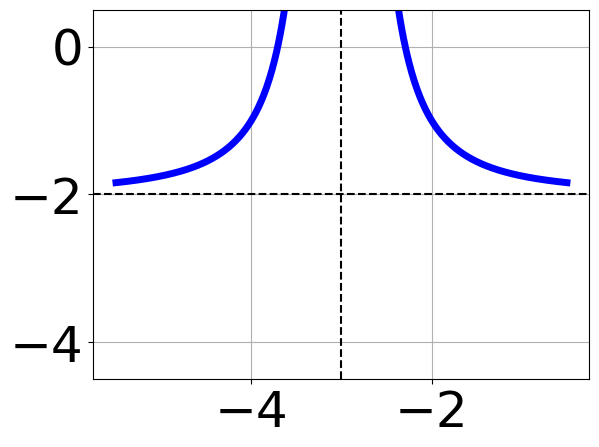
\includegraphics[width=0.5\textwidth]{../Figures/rationalGraphToEquationB.png}
\end{center}


The solution is \( f(x) = \frac{-1}{(x + 2)^2} - 3 \).\begin{enumerate}[label=\Alph*.]
\textbf{Plausible alternative answers include:}Corresponds to thinking the graph was a shifted version of $\frac{1}{x}$, using the general form $f(x) = \frac{a}{(x+h)^2}+k$, and the opposite leading coefficient.
Corresponds to using the general form $f(x) = \frac{a}{(x+h)^2}+k$ and the opposite leading coefficient.
Corresponds to thinking the graph was a shifted version of $\frac{1}{x}$.
This is the correct option.
This corresponds to believing the vertex of the graph was not correct.
\end{enumerate}

\textbf{General Comment:} Remember that the general form of a basic rational equation is $ f(x) = \frac{a}{(x-h)^n} + k$, where $a$ is the leading coefficient (and in this case, we assume is either $1$ or $-1$), $n$ is the degree (in this case, either $1$ or $2$), and $(h, k)$ is the intersection of the asymptotes.
}
\litem{
Sketch a graph that represents the equation below.
\[ f(x) = \frac{-1}{x + 1} - 3 \]The solution is the graph below.
    \begin{center}
        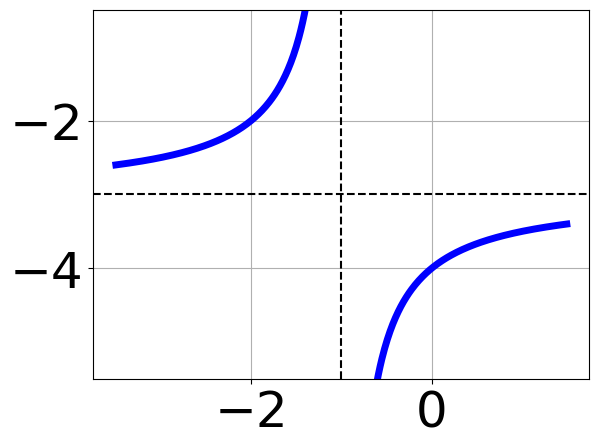
\includegraphics[width=0.3\textwidth]{../Figures/rationalEquationToGraphEB.png}
    \end{center}

\textbf{General Comment:} Remember that the general form of a basic rational equation is $ f(x) = \frac{a}{(x-h)^n} + k$, where $a$ is the leading coefficient (and in this case, we assume is either $1$ or $-1$), $n$ is the degree (in this case, either $1$ or $2$), and $(h, k)$ is the intersection of the asymptotes.
}
\litem{
Determine the domain of the function below.
\[ f(x) = \frac{4}{9x^{2} -27 x + 20} \]The solution is \( \text{All Real numbers except } x = 1.333 \text{ and } x = 1.667. \).\begin{enumerate}[label=\Alph*.]
\textbf{Plausible alternative answers include:}All Real numbers except $x = 12.000$ and $x = 15.000$, which corresponds to not factoring the denominator correctly.
This corresponds to thinking the denominator has complex roots or that rational functions have a domain of all Real numbers.
All Real numbers except $x = 1.333$, which corresponds to removing only 1 value from the denominator.
All Real numbers except $x = 1.333$ and $x = 1.667$, which is the correct option.
All Real numbers except $x = 12.000$, which corresponds to removing a distractor value from the denominator.
\end{enumerate}

\textbf{General Comment:} Recall that dividing by zero is not a real number. Therefore the domain is all real numbers \textbf{except} those that make the denominator 0.
}
\litem{
Solve the rational equation below.
\[ \frac{-2x}{-6x + 5} + \frac{-5x^{2}}{30x^{2} -43 x + 15} = \frac{-4}{-5x + 3} \]The solution is \( \text{There are two solutions: } x = 0.764 \text{ and } x = 5.236 \).\begin{enumerate}[label=\Alph*.]
\textbf{Plausible alternative answers include:}* $x = 0.764 \text{ and } x = 5.236$, which is the correct option.




\end{enumerate}

\textbf{General Comment:} Distractors are different based on the number of solutions. Remember that after solving, we need to make sure our solution does not make the original equation divide by zero!
}
\litem{
Write an equation that can represent the function graphed below.

\begin{center}
    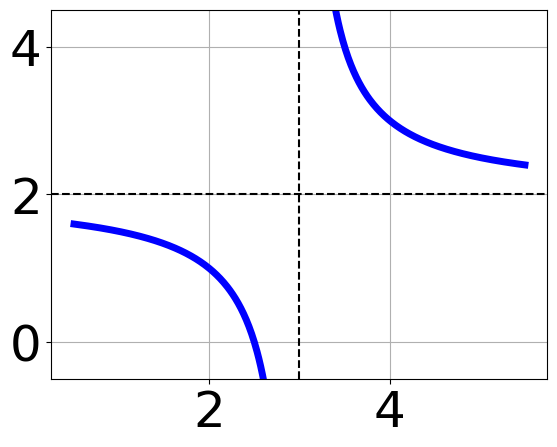
\includegraphics[width=0.5\textwidth]{../Figures/rationalGraphToEquationCopyB.png}
\end{center}


The solution is \( f(x) = \frac{1}{x - 3} + 2 \).\begin{enumerate}[label=\Alph*.]
\textbf{Plausible alternative answers include:}This is the correct option.
Corresponds to thinking the graph was a shifted version of $\frac{1}{x^2}$, using the general form $f(x) = \frac{a}{x+h}+k$, and the opposite leading coefficient.
Corresponds to thinking the graph was a shifted version of $\frac{1}{x^2}$.
Corresponds to using the general form $f(x) = \frac{a}{x+h}+k$ and the opposite leading coefficient.
This corresponds to believing the vertex of the graph was not correct.
\end{enumerate}

\textbf{General Comment:} Remember that the general form of a basic rational equation is $ f(x) = \frac{a}{(x-h)^n} + k$, where $a$ is the leading coefficient (and in this case, we assume is either $1$ or $-1$), $n$ is the degree (in this case, either $1$ or $2$), and $(h, k)$ is the intersection of the asymptotes.
}
\litem{
Sketch a graph that represents the equation below.
\[ f(x) = \frac{1}{x - 2} - 3 \]The solution is the graph below.
    \begin{center}
        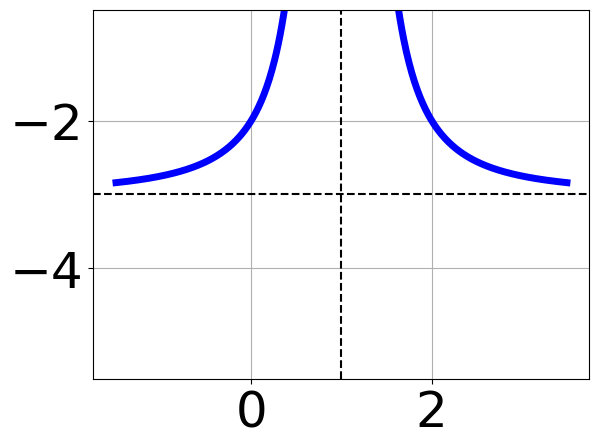
\includegraphics[width=0.3\textwidth]{../Figures/rationalEquationToGraphCopyAB.png}
    \end{center}

\textbf{General Comment:} Remember that the general form of a basic rational equation is $ f(x) = \frac{a}{(x-h)^n} + k$, where $a$ is the leading coefficient (and in this case, we assume is either $1$ or $-1$), $n$ is the degree (in this case, either $1$ or $2$), and $(h, k)$ is the intersection of the asymptotes.
}
\end{enumerate}

\end{document}